\documentclass{article}
\usepackage{hyperref}
\usepackage{float}
\usepackage{subcaption}
\usepackage{graphicx}
\graphicspath{{./images/}}

\title{Experimenting Boids algorithm with OpenGL and Vulkan API}
\author{Nicolas Ballet}
\date{\today}

\begin{document}
\maketitle
\tableofcontents
\newpage
\section{Introduction}
This project takes place during the Great Lockdown of 2020. Being in lay-off, I had plenty of time to experiment and learn new stuff.
I saw this video of Smarter Every Day: \url{https://www.youtube.com/watch?v=4LWmRuB-uNU}\\
In this video Destin talks about the flocking behavior of birds. This is quite beautiful and mesmerizing. And he shows how to simulate this kind of behavior using the Boid algorithm (Bird-droid).\\
There is three rules in this algorithm (from Wikipedia):
\begin{itemize}
    \item cohesion: steer to move towards the average position (center of mass) of local flockmates
    \item alignment: steer towards the average heading of local flockmates
    \item separation: steer to avoid crowding local flockmates
\end{itemize}
To that, I added a speed limit, and a screen-space restriction so that the boids stays inside the window.\\

But my first impression was that the number of simulation entity shown in the video was pretty low (200 boids).\\
So I searched for other examples of simulations, but I didn't find that much results.

To give some perspective to the following values here is a quick sum-up of my current hardware:
\begin{itemize}
    \item CPU: AMD Ryzen 7 3700x 3.6GHz
    \item RAM: G.Skill 32Go 3200MHz CL16
    \item GPU: AMD Radeon RX 570 4GD5
\end{itemize}
Moreover I consider that under 30 frame per second is not enough to be considered fluid, so the boids population size limit is capture so that it runs above 30fps.

\section{OpenGL prototype}
At this time, I hadn't touched OpenGL for quite a long time, this was the perfect occasion to get back to it.\\
One of the few things in OpenGL I didn't know how to use was the compute shaders.\\
When using graphical API like OpenGL or Vulkan, we tell the GPU to do some processing and sometimes we don't need the result to be displayed, so we don't need the full standard rendering pipeline. That is what compute shaders are for. Simple highly parallel processing.\\

Firstly I tried to store the boids positions inside a texture, (not knowing about Buffer Storage, which is a cleaner solution), using a compute shader to update the positions and speed vector. It worked, I reached a few thousands boids quite rapidly. But the major issue in this implementation is the fact that every boid needs to compute it's distance to every other boid to check if it is inside its visual range.\\
This is exponential, and it creates a bottleneck around 5000 boids.\\
\begin{figure}[H]
    \centering
    \begin{subfigure}[H]{\textwidth}
        \centering
        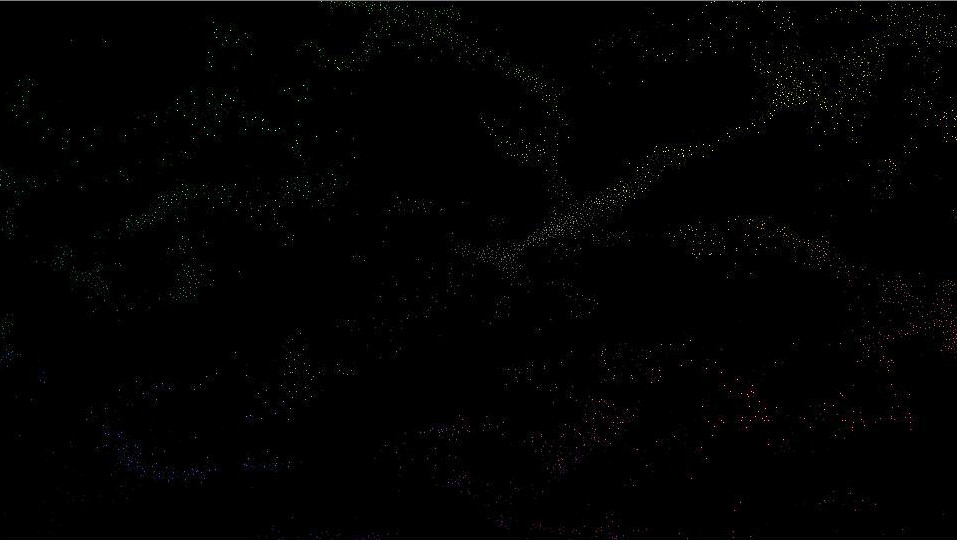
\includegraphics[width=.9\linewidth]{boids_positions.jpg}
        \caption{Boids positions on screen}
    \end{subfigure}
    \begin{subfigure}[H]{\textwidth}
        \centering
        
\includegraphics[width=.4\linewidth]{boids_positions_texture.jpg}
        \caption{Texture where boids positions are stored}
    \end{subfigure}
    \caption{Visualization of boids position storage}
\end{figure}

I then tried a little work-around by using a screen-space texture to store a kind of heatmap that I will call a vector map. I added another compute shader whose role was: for each boid, affecting the texture so that every point in the visual range of the boid represents it's "push/pull force".\\
If multiples boid visual range overlap, the resulting vector should be averaged.\\
And in the boids position update shader, I could then use the texture to get the forces applied to each boid and move there position according to that, without the need to check every other boid.\\
Here is a capture of the vector map
\begin{figure}[H]
    \centering
    \begin{subfigure}[H]{\textwidth}
        \centering
        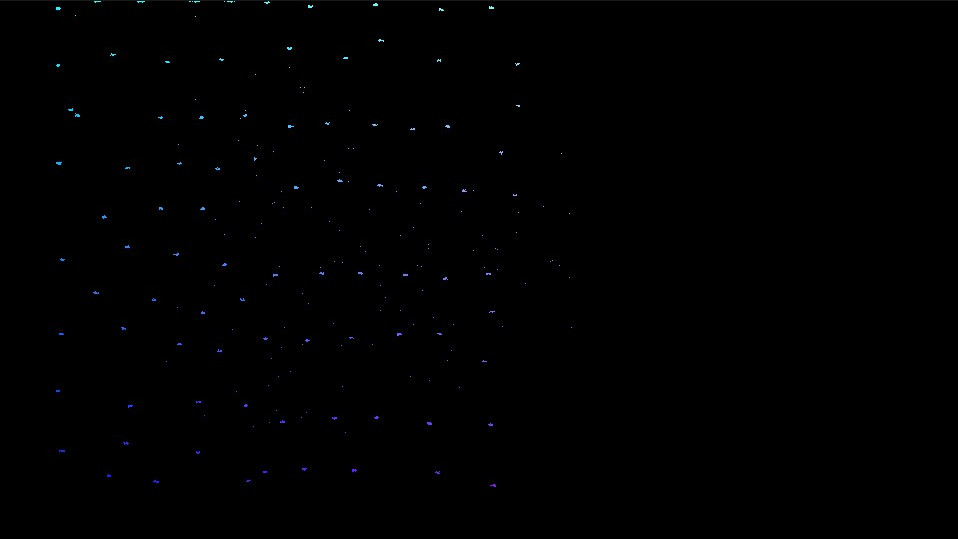
\includegraphics[width=.9\linewidth]{boids_vector_map.jpg}
        \caption{Render output of the boid positions}
    \end{subfigure}
    \begin{subfigure}[H]{\textwidth}
        \centering
        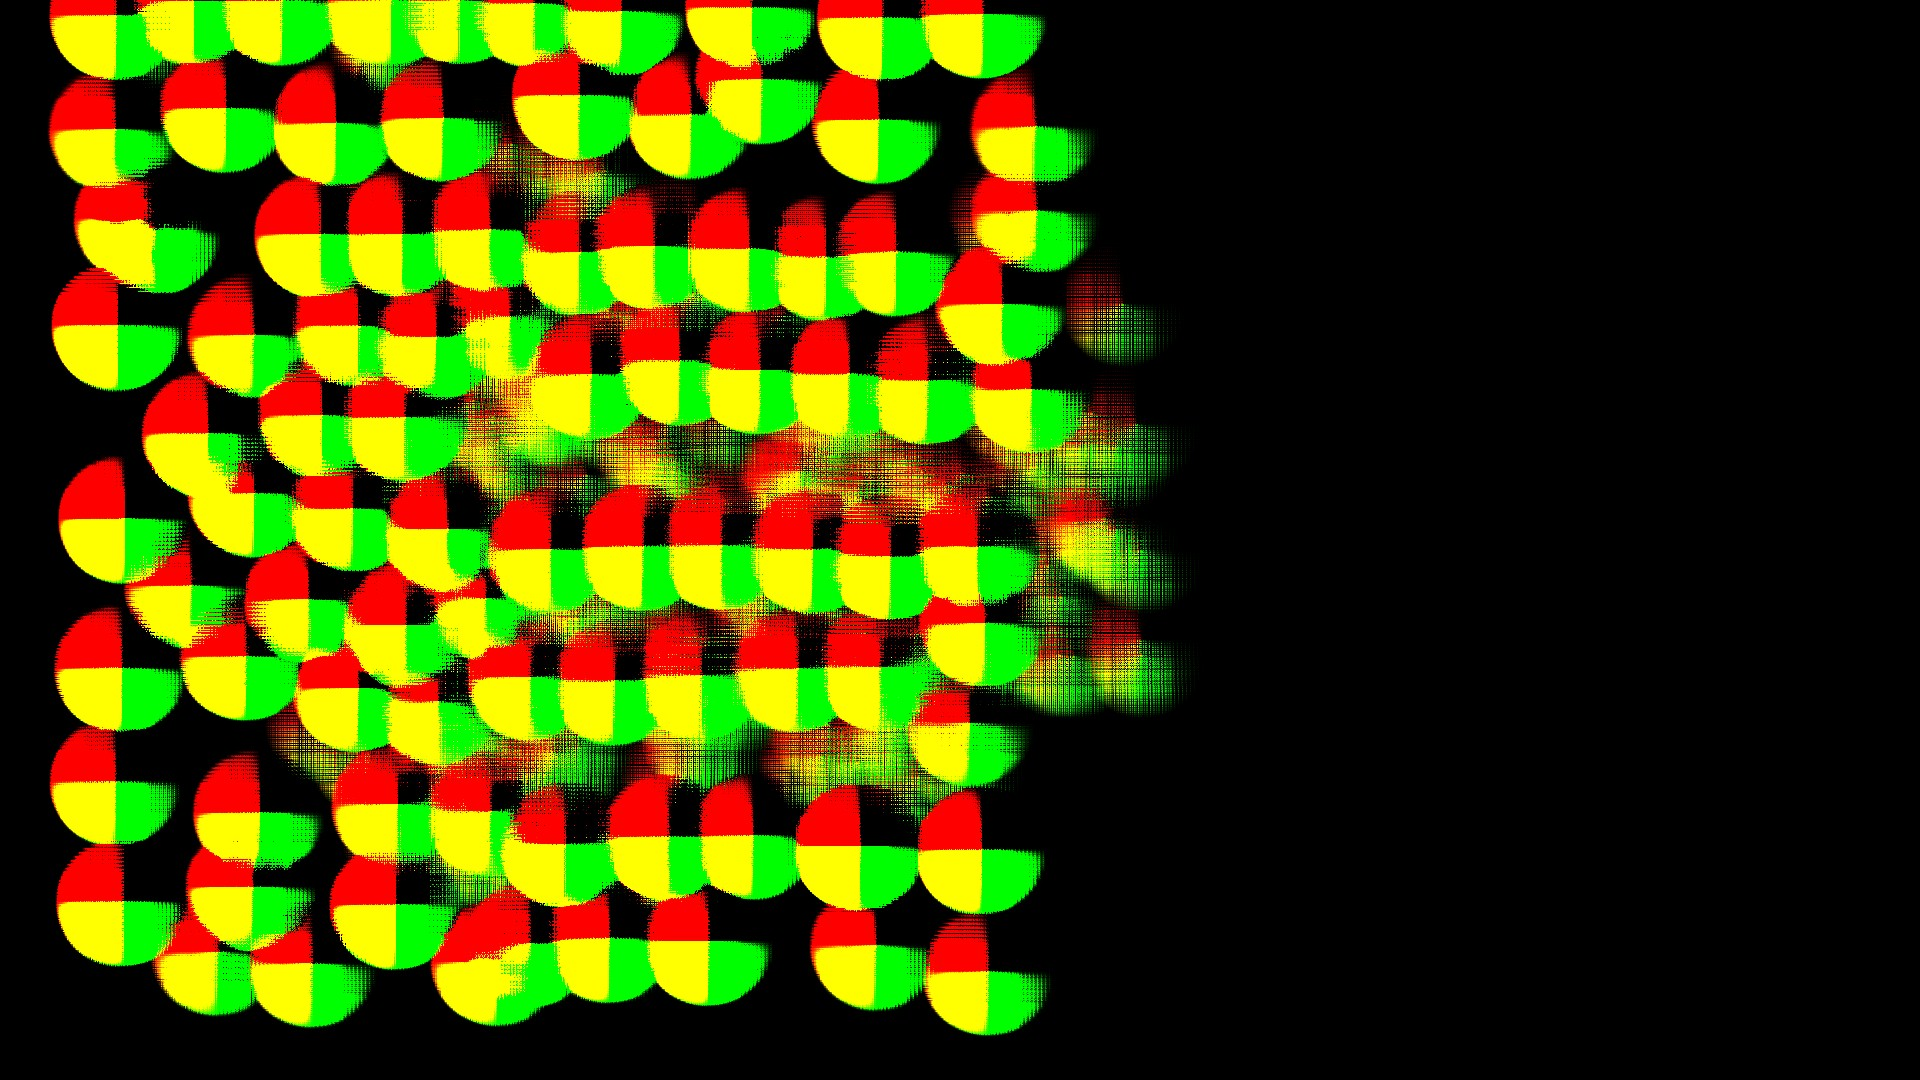
\includegraphics[width=.9\linewidth]{vector_map.jpg}
        \caption{Vector map of the push/pull forces}
    \end{subfigure}
    \caption{Visualization of the generated vector map}
\end{figure}

Besides the fact that this solution works and that I could easily make the population reach 20 thousands boids, this is no longer creating a flocking effect, this is more gravitational-like behavior.
And in top of that, as the shader execution is highly parallel, there is some race when two boids visual range overlap. And if the first one read the current value of the vector map and another stores a new value before the first boid does, the resulting value is incorrect. But as the results were not satisfying enough anyway, I dumped this work-around.\\

Finally, by looking for some references on the Internet, I read about Buffer Storage. It allows me to store the boids positions and speed vectors inside a buffer inside the graphic card, like before but without the need to extract from a texture, just a simple array.\\
Another main advantage of using Buffer Storage is that I can simply call the render pipeline with this buffer used as vertex positions and so stop using a post-processing type of render where every pixel of the image is explicitly rendered through the pipeline even if there is no boid here.\\
This doesn't change much in terms of performances, but it is cleaner and easier to understand by reading the code.

\section{Vulkan prototype}
At this point I still wanted to go higher and it was an occasion to finally try Vulkan.\\
I followed tutorials a while ago, so I approximatively knew the architecture of Vulkan but I had never really used it.\\
It was quite hard to get into, but once I isolated the few blocks I needed to work with, it was much simpler.\\
I took the sources of the tutorial I used to follow: \url{https://vulkan-tutorial.com} for the rendering side and applied about the same solution I used for OpenGL, using a Buffer Storage for the boids positions and speed vectors and using it as a Vertex Input for the render pass.\\

To create the compute shader, I used a blog called Duskborn: \url{https://www.duskborn.com/posts/a-simple-vulkan-compute-example}.\\
And just by switching to Vulkan I reached one hundred thousands boids.\\

With that many boids, scanning every boids may be mathematically perfect but computationally heavy, so I added a small hack to divide the number of flockmates each boid will check. This create small behavior artifacts if a too high factor is used but permits to reach one million boids.\\
I was done.
\begin{figure}[H]
    \centering
    \begin{subfigure}[H]{\textwidth}
        \centering
        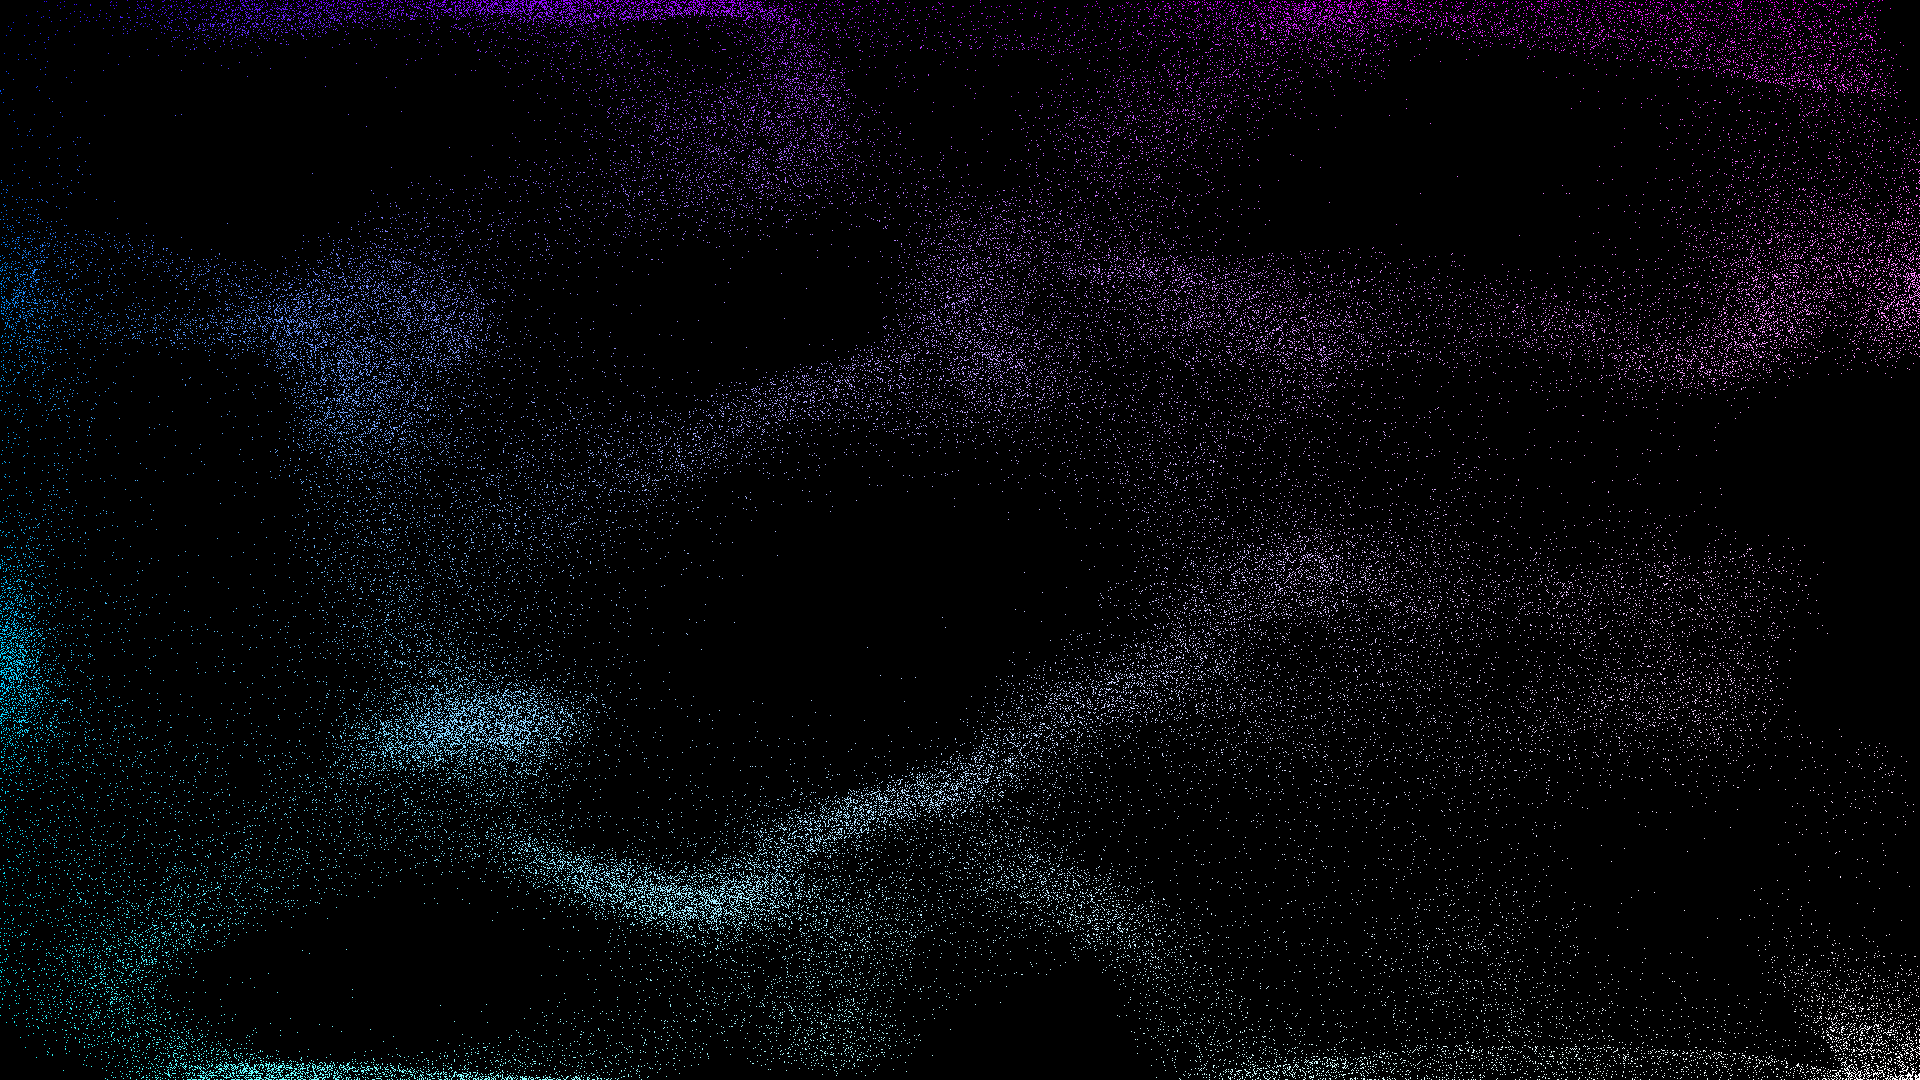
\includegraphics[width=.9\linewidth]{100000.png}
        \caption{One hundred thousands boids with no tweak.}
    \end{subfigure}
    \begin{subfigure}[H]{\textwidth}
        \centering
        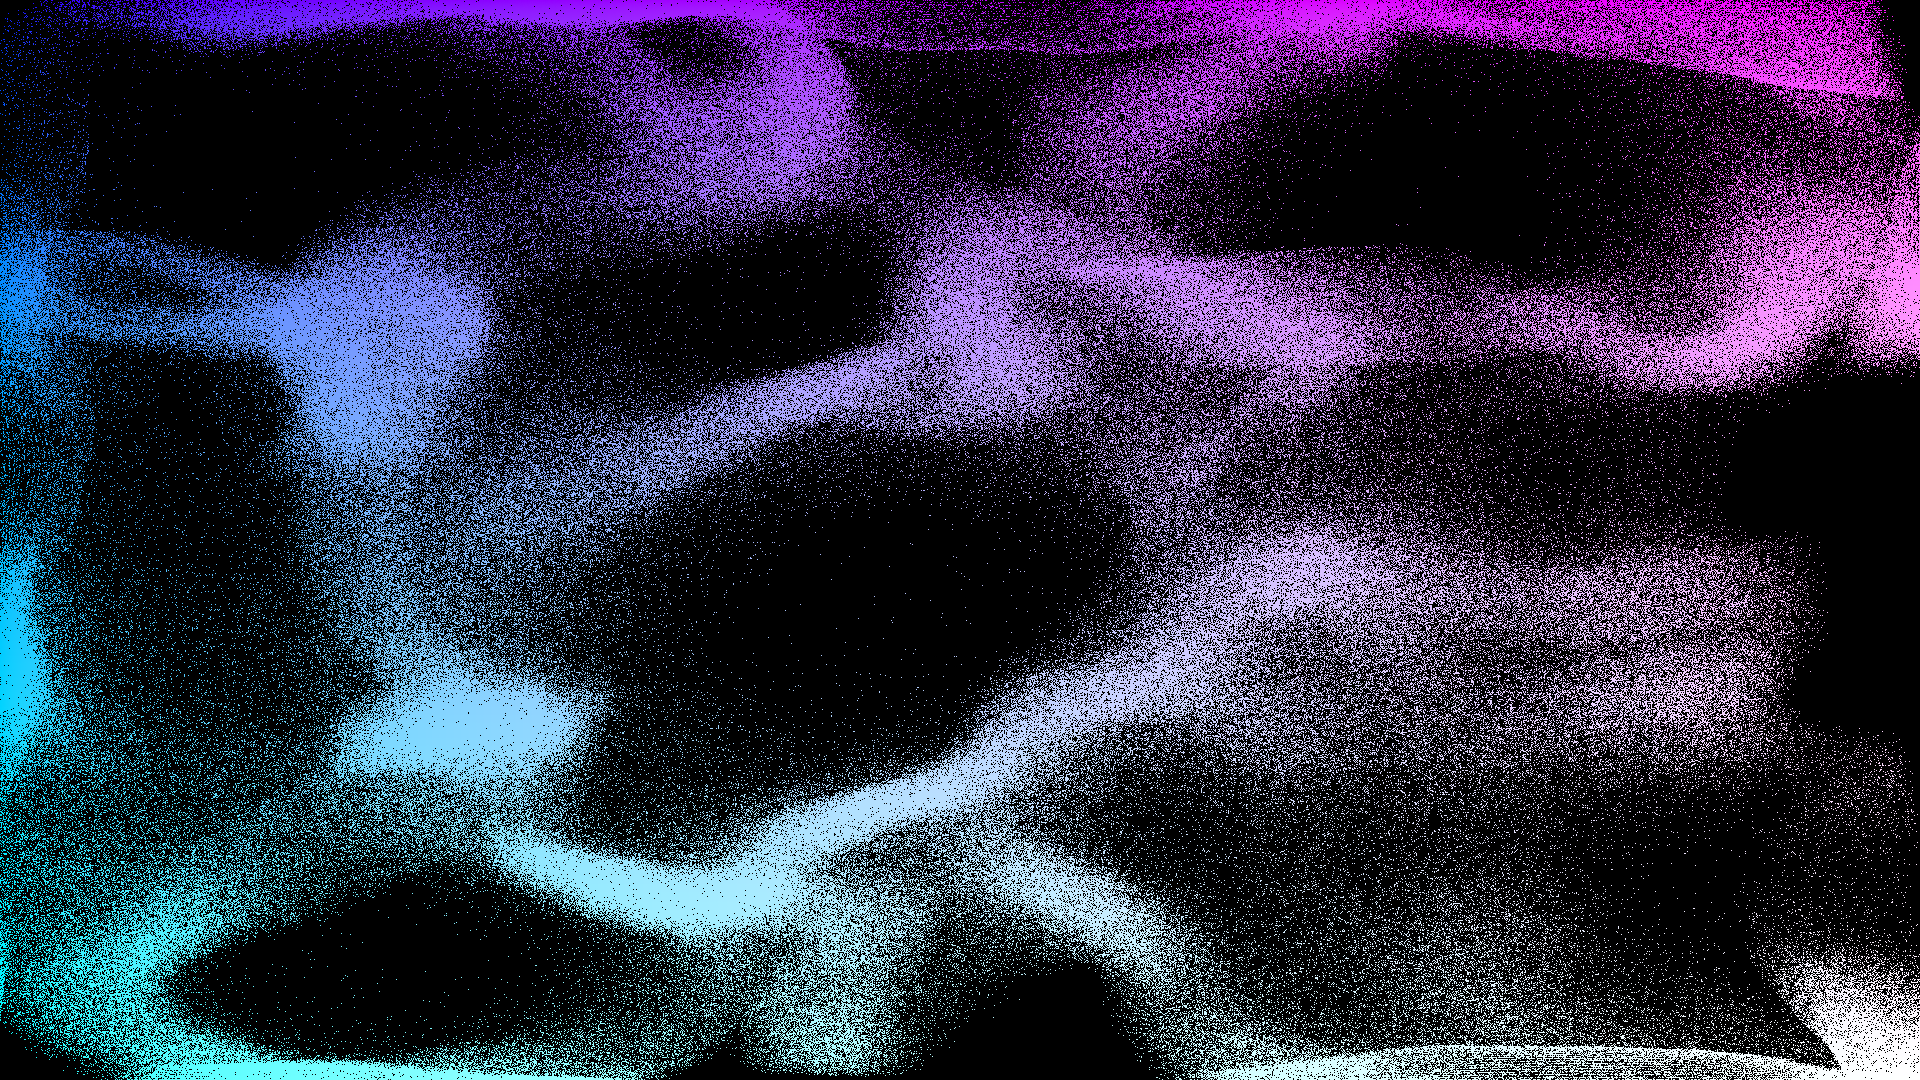
\includegraphics[width=.9\linewidth]{1000000.png}
        \caption{One million boids with a check division factor of 100.}
    \end{subfigure}
    \caption{Examples of the final results}
\end{figure}

\newpage
\section{Conclusion}
My small journey through this algorithm was quite satisfying thanks to the very cool visuals.\\
It was very interesting to develop and it allowed me to progress both with OpenGL and with Vulkan.\\
I am now much more at ease with Vulkan API and will continue to work with it.\\

I have to note down one major downside with using Vulkan for prototyping: my OpenGL version was around 230 lines of source code against the Vulkan version which was around 1700 lines of code.\\
From this experience, I think that prototyping the first versions with OpenGL and then using Vulkan to validate the performances is a great workflow, at least for some non-expert like me.

\newpage
\listoffigures
\end{document}
